\title{QuantEx: Interim Report 1}
\author{
        QuantEx Team at ICHEC
}
\date{\today}

\documentclass[12pt]{article}
\usepackage{amsmath}
\usepackage[usenames, dvipsnames]{xcolor}
\usepackage{listings}
\usepackage{url}

\lstdefinelanguage{Julia}
  {morekeywords={abstract,break,case,catch,const,continue,do,else,elseif,
      end,export,false,for,function,immutable,import,importall,if,in,
      macro,module,otherwise,quote,return,switch,true,try,type,typealias,
      using,while},
   sensitive=true,
   alsoother={\$},
   morecomment=[l]\#,
   morecomment=[n]{\#=}{=\#},
   morestring=[s]{"}{"},
   morestring=[m]{'}{'},
}[keywords,comments,strings]

\lstset{
    language         = Julia,
    basicstyle       = \ttfamily,
    keywordstyle     = \bfseries\color{blue},
    stringstyle      = \color{magenta},
    commentstyle     = \color{ForestGreen},
    showstringspaces = false,
}

% additional packages
\usepackage{tikz-network}
\usepackage{listings}
\usepackage[braket, qm]{qcircuit}
\usepackage{amsmath}

\begin{document}
\maketitle

\begin{abstract}
Working document for first QuantEx interim report in which we keep track of
background reading, exploration work and planning process to arrive at initial
prototype design.
\end{abstract}

\section{Introduction}
In this report we track the progress of the initial stages of the QuantEx project. In section \ref{evaluations} report on evaluations of the currently existing tools and methods for simulating quantum circuits using tensor networks. For each, we assess their potential to be integrated and/or modified to form part of the QuantEx toolset and to scale to emerging exa-scale compute platforms. In section \ref{design} we outline the interfaces and architecture of each layer that will be used for the initial implementation.

% include section on evaluations
\section{Evaluations}\label{evaluations}
Here we go through each of the relevant packages and assess their applicability for use in the QuantEx project.

\subsection{cuTENSOR} \label{cutensor}
cuTENSOR\cite{cuTENSOR} is a high performance CUDA library for tensor primitives, with support for tensors of up to rank 12. In cuTENSOR, a tensor is an n-dimensional array that is described by:

\begin{itemize}
\item Its rank i.e.\ the number of modes
\item The extent of each mode
\item Its strides, which are inferred if unspecified
\item Its datatype
\item A unary operation (e.g.\ \texttt{CUTENSOR\_OP\_IDENTITY}) applied to each element
\end{itemize}

\noindent Some of the library's key features, which will be discussed below, include:

\begin{itemize}
\item Element-wise operations
\item Tensor reductions
\item Direct contraction operations (i.e. transpose-free contraction)
\end{itemize}

\noindent For brevity, full CUDA code samples have been omitted here. Detailed examples of element-wise operations, reductions, and contractions may be found in NVIDIA's CUDA library samples git repo\footnote{\url{https://github.com/NVIDIA/CUDALibrarySamples}}. It is to be noted that cuTENSOR requires a relatively new NVIDIA GPU with compute capability of 7.0.


\subsubsection{Element-wise operations} \label{cutensor::elementwise}
There are three element-wise operations provided by cuTENSOR, which will be summarised here.

\vspace{0.5em}\texttt{cutensorPermutation}: performs out-of-place tensor permutations of the form

\begin{equation*} 
B_{\Pi^B(i_0,i_1,...,i_n)} = \alpha\Psi(A_{\Pi^A(i_0,i_1,...,i_n)}),
\end{equation*}

\noindent where $A$ and $B$ are tensors, $\Pi^A$ and $\Pi^B$ are permutation operations that permute the indices of $A$ and $B$, and $\Psi$ is a unary, element-wise operation, such as \texttt{CUTENSOR\_OP\_IDENTITY} or \texttt{CUTENSOR\_OP\_CONJ}, that is specified in the tensor description of $A$.

\vspace{0.5em}\texttt{cutensorElementwiseBinary}: performs the following element-wise operation for two input tensors:

\begin{equation*}
D_{\Pi^C(i_0,i_1,...,i_n)} = \Phi_{AC}(\alpha\Psi_A(A_{\Pi^A(i_0,i_1,...,i_n)}), \gamma\Psi_C(C_{\Pi^C(i_0,i_1,...,i_n)})),
\end{equation*}

\noindent with the notation as described above and $\Phi_{AC}$ being a binary operation such as \texttt{CUTENSOR\_OP\_ADD} or \texttt{CUTENSOR\_OP\_MAX}.

\vspace{0.5em}\texttt{cutensorElementwiseTrinary}: allows a more complex tensor operation that is applied to three input tensors:

\begin{multline*}
D_{\Pi^C(i_0,i_1,...,i_n)} = \Phi_{ABC}(
  \Phi_{AB}(
    \alpha\Psi_A(A_{\Pi^A(i_0,i_1,...,i_n)}),
    \beta\Psi_B(B_{\Pi^B(i_0,i_1,...,i_n)})
  ),\\
  \gamma\Psi_C(C_{\Pi^C(i_0,i_1,...,i_n)})
).
\end{multline*}

\noindent Some example operations of what can be achieved with \texttt{cutensorElementwi\-seTrinary}:
\begin{itemize}
\item $D_{a,b,c,d} = A_{b,d,a,c}$
\item $D_{a,b,c,d} = 2.2 \times A_{b,d,a,c} + 1.3 \times B_{c,b,d,a}$
\item $D_{a,b,c,d} = 2.2 \times A_{b,d,a,c} + 1.3 \times B_{c,b,d,a} + C_{a,b,c,d}$
\item $D_{a,b,c,d} = \mathrm{min}((2.2 \times A_{b,d,a,c} + 1.3 \times B_{c,b,d,a}), C_{a,b,c,d})$
\end{itemize}

\subsubsection{Reduction operations} \label{cutensor::reduction}
The following is a summary of the reduction operations provided by cuTENSOR:

\vspace{0.5em}\texttt{cutensorReduction}: performs general reductions of the form:

\begin{equation*}
D = \alpha \times \mathrm{opReduce}(\Psi_A(A)) + \beta \Psi_C(C).
\end{equation*}

\noindent $\mathrm{opReduce}$ is a binary operation that is used to reduce the elements of $A$. For example, using \texttt{CUTENSOR\_OP\_ADD} will sum over the elements of $\Psi_A(A)$, while \texttt{CUTENSOR\_OP\_MAX} will give the maximum element of $\Psi_A(A)$.

The reduction operation may require some additional scratchpad memory on the device in order to complete. Therefore, the \texttt{cutensorReduction} function has two additional arguments: one being a pointer to the device scratchpad memory and the other being its size. The scratchpad size need not be calculated manually; one may use the \texttt{cutensorReductionGetWorkspace} helper function, which assesses the reduction to be performed using the tensor descriptions and computes the required size. A device buffer of this size must be allocated manually and the resulting pointer passed to \texttt{cutensorReduction}.

Furthermore, partial reductions may be carried out by only specifying a subset of indices:

\begin{equation*}
D_{i,j} = \alpha \times \mathrm{opReduce}(A_{i,j,k}).
\end{equation*}

\subsubsection{Contraction operations} \label{cutensor::contraction}
Following is a summary of the contraction operations provided by cuTENSOR, including functions required to prepare a contraction.

\vspace{0.5em}\texttt{cutensorInitContractionDescription}: this is used to initialise a contraction description object, of type \texttt{cutensorContractionDescriptor\_t}, \\where the tensor contraction is of the form

\begin{equation*}
D_{\mathrm{modes}_D} = \alpha A_{\mathrm{modes}_A} B_{\mathrm{modes}_B} + \beta C_{\mathrm{modes}_C},
\end{equation*}

\noindent using the descriptions of the input tensors $A$, $B$, and $C$, and the output tensor $D$.

\vspace{0.5em}\texttt{cutensorInitContractionFind}: this function may be used to limit the search space of potential contraction algorithms that \texttt{cutensorInitContr\-actionPlan} is allowed to evaluate. \texttt{CUTENSOR\_ALGO\_DEFAULT} lets the heuristic choose the algorithm while other possible options include:

\begin{itemize}
\item \texttt{CUTENSOR\_ALGO\-\_GETT} -- GEMM-like Tensor-Tensor multiplication\footnote{\url{https://dl.acm.org/doi/10.1145/3157733}}
\item \texttt{CUTENSOR\_ALGO\_TGETT} -- Transpose A or B + GETT
\item \texttt{CUTENSOR\_ALGO\_TTGT} -- Transpose-Transpose-GEMM-Transpose
\end{itemize}


\vspace{0.5em}\texttt{cutensorContractionGetWorkspace}: similarly to the reduction case, this helper function is used to determine the required scratch space for a given tensor contraction.

\vspace{0.5em}\texttt{cutensorInitContractionPlan}: initialise the contraction plan for the described contraction on the currently active device. cuTENSOR’s heuristic is used to select a candidate plane for a given tensor contraction. As with other libraries, such as FFTW, this plan may be reused multiple times as long as the described contraction remains the same.


\vspace{0.5em}\texttt{cutensorContraction}: performs the planned contraction as set up using \texttt{cutensorInitContractionDescription}. This has the requirement that the active device at kernel invocation is the same one that was active when the plan was initialised.


\vspace{0.5em}\texttt{cutensorContractionMaxAlgos}: this function is used to compute the maximum number of algorithms available to compute tensor contractions\footnote{This function takes no information of the contraction problem so I suspect that perhaps this function is used to probe the capability of the underlying hardware.}. In the case that an algorithm isn't supported, \texttt{cutensorContraction} will return \texttt{CUTENSOR\_STAT\-US\_NOT\_SUPPORTED}. This may be used as an optimisation step in preparing a number of identical contractions, see Listing~\ref{cutensor::optim_example}.

\begin{lstlisting}[language=C++, label=cutensor::optim_example, basicstyle=\small, caption=Finding the most efficient 
algorithm]

int32_t maxAlgosTC = 0;
cutensorContractionMaxAlgos(&maxAlgosTC);

float min_time = std::numeric_limits<float>::max();
int first_algo = static_cast<int>(CUTENSOR_ALGO_GETT);
for (int algo = first_algo; algo < maxAlgosTC; algo++) {
  // Plan and execute contraction using algo measuring
  // the time taken
  
  if (time_taken < min_time) {
    min_time = time_taken;
    optim_algo = algo;
  }
}

// Continue using optim_algo
\end{lstlisting}

\subsubsection{cuTENSOR Contraction Workflow} \label{cutensor::workflow}
The general workflow for completing a tensor contraction is outlined below. The documentation for each library function mentioned, as well as a tensor contraction example code, can be found at \url{https://docs.nvidia.com/cuda/cutensor/api/cutensor.html}.

\begin{enumerate}
\item Create array of indices for each tensor
\item Create map of indices to extents i.e. the size of each labelled dimension
\item Create array of extents for each tensor
\item Copy each tensor to the device
\item Initialise the cuTENSOR library - \texttt{cutensorInit}
\item Create descriptor for each tensor using its size, extents, and a unary operation - \texttt{cutensorInitTensorDescriptor}
\item Compute the necessary alignment for each tensor - \texttt{cuTensorGetAlign\-mentRequirement}
\item Create descriptor for the contraction using the tensor descriptors - \texttt{cutensorInitContractionDescriptor}
\item Find contraction plan - \texttt{cutensorInitContractionFind}
\item Compute the necessary workspace - \texttt{cutensorContractionGetWorksp\-ace}
\item Initialise contraction plan - \texttt{cutensorInitContractionPlan}
\item Execute contraction - \texttt{cutensorContraction}
\item Copy results back to the host
\end{enumerate}

\subsubsection{TensorOperations.jl Integration} \label{cutensor::julia}
cuTENSOR has been integrated into the TensorOperations.jl\footnote{\url{https://github.com/Jutho/TensorOperations.jl}} Julia package. This allows the offloading of tensor contractions to the GPU using similar syntax to the standard TensorOperations contractions, with the difference being the use of the \texttt{@cutensor} macro in place of \texttt{@tensor}. The use of this macro will transfer all arrays to the device before contraction. An example is shown in Listing~\ref{cutensor::julia_example}.

\begin{lstlisting}[language=Julia, label=cutensor::julia_example, caption=cuTENSOR contraction in Julia]
using CuArrays
using TensorOperations

alpha = randn(Float32);
A = randn(Float32,5,5,5,5,5,5);
B = randn(Float32,5,5,5);
C = randn(Float32,5,5,5);
D = zeros(Float32,5,5,5);

@cutensor D[a,b,c] = A[a,e,f,c,f,g]*B[g,b,e] +
			alpha*C[c,a,b]
@cutensor E[a,b,c] := A[a,e,f,c,f,g]*B[g,b,e] +
			alpha*C[c,a,b]
\end{lstlisting}

\noindent In Listing~\ref{cutensor::julia_example}, since the array \texttt{D} exists on the host, it will be copied back at the end of the operation. As \texttt{E} does not, it will remain on the device for further operation. It is to be noted that mixed operations between host and device arrays will fail. Also, as shown in Listing~\ref{cutensor::julia_example}, it is necessary to import CuArrays as failing to do so will raise an error that \texttt{@cutensor} is undefined.

\subsubsection{Future Research} \label{cutensor::futurework}
The following will need to be looked into going forward:

\begin{enumerate}
\item Benchmark cuTENSOR's integration in TensorOperations.jl
\item Operations that don't fit in device memory and investigate further limitations of cuTENSOR
\item Multi-GPU operations
\end{enumerate}

\subsection{qflex}
The qflex simulator received a lot of attention for its use in the google quantum supremacy experiments \cite{Villalonga2019} and managed to reach sustained performance of 281 Pfops/s on the Summit supercomputer at Oakridge National Laboratory.... 



% include section on design of initial implementation
\section{Design of initial implementation}\label{design}
Here we document the initial design for QuantEx. For separation of concerns we
divide QuantEx into three distinct layers as shown in figure \ref{fig:layers}.

\begin{figure}\label{fig:layers}
\centering
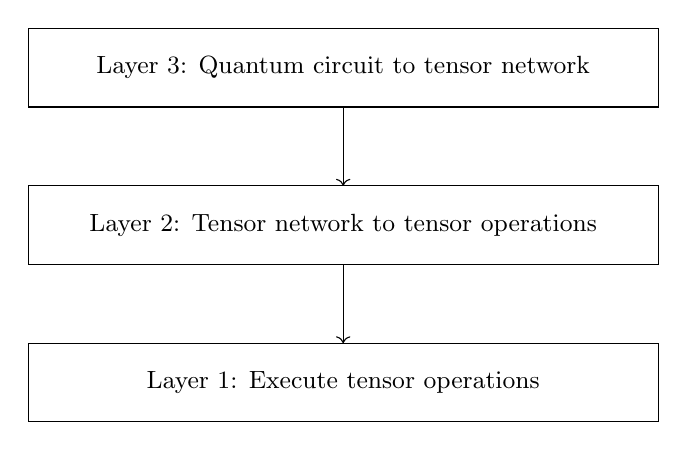
\begin{tikzpicture}
  \draw (0, 4) rectangle (8, 5);
  \node at (4, 4.5) {\small Layer 3: Quantum circuit to tensor network};
  \draw [->] (4, 4) -- (4, 3);

  \draw (0, 2) rectangle (8, 3);  
  \node at (4, 2.5) {\small Layer 2: Tensor network to tensor operations};
  \draw  [->] (4, 2) -- (4, 1);
    
  \draw (0, 0) rectangle (8, 1.0);
  \node at (4, 0.5) {\small Layer 1: Execute tensor operations};
\end{tikzpicture}
\caption{High level QuantEx architcture}
\end{figure}

\subsection{Layer 3: Quantum circuit to tensor network}
The highest level layer is responsible for converting an arbitrary quantum circuit to
a tensor network. The quantum assembly language (QASM) \cite{cross2017open}
is used as the format for describing quantum circuits. Using this open standard
format enables interoperability with the many available quantum computing
frameworks. We demonstrate each step here with an example circuit which
prepares a three qubit GHZ state. The circuit for preparing this state consists
of a Hadamard gate applied to the first qubit followed by controlled not gates
applied to the first and second and second and third qubits respectively. The
circuit is shown below and the QASM code describing this circuit is given in
listing \ref{lst:ghz_qasm}.

\begin{equation}\label{eqn:ghz_circuit}
    \Qcircuit @C=1.0em @R=0.0em @!R {
	 	\lstick{ q_{0} : \ket{0} } & \gate{H} & \ctrl{1} & \qw & \qw & \qw\\
	 	\lstick{ q_{1} : \ket{0} } & \qw & \targ & \ctrl{1} & \qw & \qw\\
	 	\lstick{ q_{2} : \ket{0} } & \qw & \qw & \targ & \qw & \qw\\
	 }
\end{equation}

\begin{minipage}{\linewidth}
\begin{lstlisting}[caption={QASM for three qubit GHZ preparation},label={lst:ghz_qasm}]
OPENQASM 2.0;
include "qelib1.inc";
qreg q[3];
h q[0];
cx q[0],q[1];
cx q[1],q[2];
\end{lstlisting}
\end{minipage}

\subsubsection{Tensor Network Notation and Conventions}
One of the trickier aspects of working with tensor networks is keeping track of
indices. Using graphical notation and maintaining consistency in how links
are labeled helps avoid confusion and prevent errors. Here we
present a short introduction to tensor networks, their graphical notation and
the index labeling conventions we will adopt for QuantEx. There are many
excellent resources for further reading on tensor networks and their use in
quantum information, for example see \cite{biamonte2017tensor, Bridgeman_2017, wood2011tensor}.

A tensor is a multi-dimensional array of numbers, where the rank gives the
number of dimensions. Graphically a tensor can be represented by a node with an
edge for each dimension. Figure \ref{fig:vector_matrix_tensors} shows how
vectors and matrices are represented graphically. Column vectors (or kets) have
an open link pointing to the right and row vectors (or bras) have an open link
pointing to the right.

An edge between tensors indicates contraction over the connected indices. Figure
\ref{fig:basic_tensor_contractions} shows how an inner product between two
vectors and a matrix vector multiplication are represented graphically. Using
this notation, we can represent quantum circuits graphically as tensor
networks. The three qubit GHZ preparation circuit shown in \ref{eqn:ghz_circuit}
can be represented as in figure \ref{fig:ghz_tn_circuit}.

\begin{figure}\label{fig:vector_matrix_tensors}
\centering
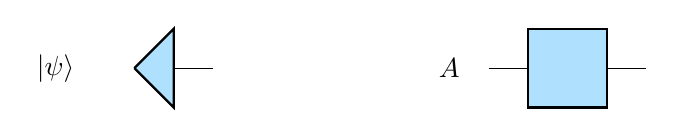
\begin{tikzpicture}
  \definecolor{lightblue}{RGB}{175,225,255}
  % draw vector and ket
  \node at (0, 0) {$|\psi\rangle$};
  \draw [black, fill=lightblue, thick] (1, 0) -- (1.5, 0.5) -- (1.5, -0.5) -- (1, 0);
  \draw (1.5, 0) -- (2, 0);
  
  % draw matrix
  \node at (5, 0) {$A$};
  \draw [black, fill=lightblue, thick] (6, -0.5) rectangle (7, 0.5);
  \draw (5.5, 0) -- (6, 0);
  \draw (7, 0) -- (7.5, 0);
\end{tikzpicture}
\caption{Graphical representation of vector and matrix}
\end{figure}

\begin{figure}\label{fig:basic_tensor_contractions}
\centering
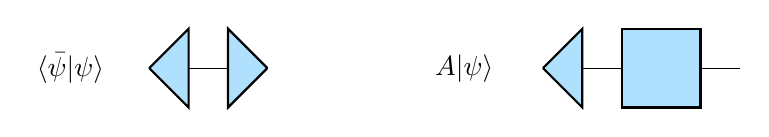
\begin{tikzpicture}
  \definecolor{lightblue}{RGB}{175,225,255}
  \node at (0, 0) {$\langle \bar{\psi} |\psi\rangle$};
  \draw [black, fill=lightblue, thick] (1, 0) -- (1.5, 0.5) -- (1.5, -0.5) -- (1, 0);
  \draw (1.5, 0) -- (2, 0);
  \draw [black, fill=lightblue, thick] (2.5, 0) -- (2, 0.5) -- (2, -0.5) -- (2.5, 0);
  
  \node at (5, 0) {$A | \psi \rangle $};
  \draw [black, fill=lightblue, thick] (6, 0) -- (6.5, 0.5) -- (6.5, -0.5) -- (6, 0);
  \draw [black, fill=lightblue, thick] (7, -0.5) rectangle (8, 0.5);
  \draw (6.5, 0) -- (7, 0);
  \draw (8, 0) -- (8.5, 0);
\end{tikzpicture}
\caption{Graphical representation of inner product and matrix vector multiplication}
\end{figure}

\begin{figure}\label{fig:ghz_tn_circuit}
\centering
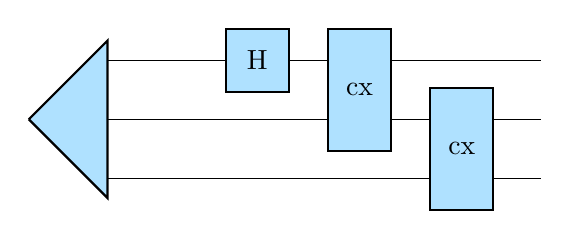
\begin{tikzpicture}
  \definecolor{lightblue}{RGB}{175,225,255}
  \draw [black, fill=lightblue, thick] (0, 0) -- (1, 1) -- (1, -1) -- (0, 0);
  \draw (1, 0.75) -- (2.5, 0.75);
  \draw [black, fill=lightblue, thick] (2.5, 0.35) rectangle (3.3, 1.15);
  \node at (2.9, 0.75) {H};
  \draw (3.3, 0.75) -- (3.8, 0.75);
  \draw (1, 0) -- (3.8, 0);
  \draw [black, fill=lightblue, thick] (3.8, -0.4) rectangle (4.6, 1.15);
  \node at (4.2, 0.375) {cx};
  \draw (4.6, 0.75) -- (6.5, 0.75);
  \draw (4.6, 0) -- (5.1, 0);
  \draw (1, -0.75) -- (5.1, -0.75);
  \draw [black, fill=lightblue, thick] (5.1, -1.15) rectangle (5.9, 0.4);
  \node at (5.5, -0.375) {cx};
  \draw (5.9, 0) -- (6.5, 0);
  \draw (5.9, -0.75) -- (6.5, -0.75);
\end{tikzpicture}
\caption{Three qubit GHZ preparation circuit as tensor network}
\end{figure}

The tensor network shown in figure \ref{fig:ghz_tn_circuit} does indeed
implement the GHZ circuit. However since the input state consists of a single
large tensor, storing this tensor requires the same amount of memory as full
wave-function methods. Breaking this large tensor into a network of smaller
tensors enables more compact representation of many states (maximally entangled
states require the same space as the full wave-function). Figure
\ref{fig:ghz_tn_mps_circuit} shows the same GHZ preparation circuit as in figure
\ref{fig:ghz_tn_circuit} but with the large input tensor broken into
individual tensors. In this case the large tensor is represented as a one
dimensional chain of tensors called a Matrix Product State (MPS). It is possible
to map the input tensor to other geometries including two or three dimensional arrays of tensors
with open/closed boundaries, fully connected networks of tensors or some
arbitrary graph. The geometry to map should be an input parameter to layer 3
with a sensible default if none is supplied. The use of the MPS representation has
particular benefits because it can be efficiently compressed
\cite{Schollw_ck_2011, zhou2020limits}.

\begin{figure}\label{fig:ghz_tn_mps_circuit}
\centering
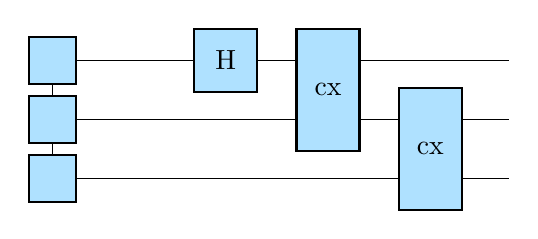
\begin{tikzpicture}
  \definecolor{lightblue}{RGB}{175,225,255}
  \draw [black, fill=lightblue, thick] (0.4, -0.3) rectangle (1.0, 0.3);
  \draw (0.7, 0.3) -- (0.7, 0.45);
  \draw [black, fill=lightblue, thick] (0.4, 0.45) rectangle (1.0, 1.05);
  \draw (0.7, -0.3) -- (0.7, -0.45);
  \draw [black, fill=lightblue, thick] (0.4, -1.05) rectangle (1.0, -0.45);
  \draw (1, 0.75) -- (2.5, 0.75);
  \draw [black, fill=lightblue, thick] (2.5, 0.35) rectangle (3.3, 1.15);
  \node at (2.9, 0.75) {H};
  \draw (3.3, 0.75) -- (3.8, 0.75);
  \draw (1, 0) -- (3.8, 0);
  \draw [black, fill=lightblue, thick] (3.8, -0.4) rectangle (4.6, 1.15);
  \node at (4.2, 0.375) {cx};
  \draw (4.6, 0.75) -- (6.5, 0.75);
  \draw (4.6, 0) -- (5.1, 0);
  \draw (1, -0.75) -- (5.1, -0.75);
  \draw [black, fill=lightblue, thick] (5.1, -1.15) rectangle (5.9, 0.4);
  \node at (5.5, -0.375) {cx};
  \draw (5.9, 0) -- (6.5, 0);
  \draw (5.9, -0.75) -- (6.5, -0.75);
\end{tikzpicture}
\caption{Three qubit GHZ preparation circuit as tensor network with a MPS used
  for the input state}
\end{figure}

\subsubsection{Tensor Network Internal Representation}

An internal representation for tensor networks is required for interchanging
tensor network descriptions between layers. Tensor networks are graphs where
nodes are tensors and edges contractions over tenor indices. For an interchange
format we require the ability to save the tensor data for each node along with
information on index ordering and edges. For this we build an internal graph
data structure and functionality convert to and from JSON format. The resulting 
JSON for a two qubit GHZ circuit is given in listing \ref{lst:ghz_json}.

\begin{lstlisting}[label=lst:ghz_json, basicstyle=\small, caption=Tensor network graph for two qubit GHZ circuit]
{
  "inputs": [
    1,
    2
  ],
  "outputs": [
    3,
    4
  ],
  "nodes": {
    "1": {
      "data_order": "col",
      "indices": [
        1
      ],
      "dims": [
        2
      ],
      "type": "input",
      "data_re": [
        1.0,
        0.0
      ],
      "data_im": [
        0.0,
        0.0
      ],
      "qubits": [
        1
      ]
    },
    "2": {
      "data_order": "col",
      "indices": [
        1
      ],
      "dims": [
        2
      ],
      "type": "input",
      "data_re": [
        1.0,
        0.0
      ],
      "data_im": [
        0.0,
        0.0
      ],
      "qubits": [
        2
      ]
    },
    "3": {
      "data_order": "col",
      "indices": [
        1
      ],
      "dims": [
        2
      ],
      "type": "output",
      "data_re": [
        1.0,
        0.0
      ],
      "data_im": [
        0.0,
        0.0
      ],
      "qubits": [
        3
      ]
    },
    "4": {
      "data_order": "col",
      "indices": [
        1
      ],
      "dims": [
        2
      ],
      "type": "output",
      "data_re": [
        1.0,
        0.0
      ],
      "data_im": [
        0.0,
        0.0
      ],
      "qubits": [
        4
      ]
    },
    "5": {
      "data_order": "col",
      "indices": [
        1,
        2
      ],
      "dims": [
        2,
        2
      ],
      "type": "gate",
      "data_re": [
        0.7071067811865475,
        0.7071067811865475,
        0.7071067811865475,
        -0.7071067811865475
      ],
      "data_im": [
        0.0,
        0.0,
        0.0,
        0.0
      ],
      "qubits": [
        0
      ]
    },
    "6": {
      "data_order": "col",
      "indices": [
        1,
        2,
        3,
        4
      ],
      "dims": [
        2,
        2,
        2,
        2
      ],
      "type": "gate",
      "data_re": [
        1.0,
        0.0,
        0.0,
        0.0,
        0.0,
        1.0,
        0.0,
        0.0,
        0.0,
        0.0,
        1.0,
        0.0,
        0.0,
        0.0,
        0.0,
        -1.0
      ],
      "data_im": [
        0.0,
        0.0,
        0.0,
        0.0,
        0.0,
        0.0,
        0.0,
        0.0,
        0.0,
        0.0,
        0.0,
        0.0,
        0.0,
        0.0,
        0.0,
        0.0
      ],
      "qubits": [
        0,
        1
      ]
    }
  },
  "edges": {
    "1": {
      "src": 1,
      "dst": 5,
      "indices": [
        1,
        1
      ]
    },
    "2": {
      "src": 2,
      "dst": 6,
      "indices": [
        1,
        2
      ]
    },
    "3": {
      "src": 5,
      "dst": 6,
      "indices": [
        2,
        1
      ]
    },
    "4": {
      "src": 6,
      "dst": 3,
      "indices": [
        3,
        1
      ]
    },
    "5": {
      "src": 6,
      "dst": 4,
      "indices": [
        4,
        1
      ]
    }
  }
}
\end{lstlisting}

\subsection{Layer 2: Tensor Network to Tensor Operations}


\subsection{Layer 1: Execute Tensor operations}

\section{Conclusions}\label{conclusions}

\bibliographystyle{habbrv}
\bibliography{library}

\end{document}
This is never printed